\newpage
\section{Усовершенствования для соседства, идеи от пользователей}

\subsection{Районы и Сообщество}

Районы постоянно развиваются, в основном новые, которые формируются, это ясно, так как многое предстоит сделать. Некоторые из них достигли большей эволюции, чем другие. В эволюции соседства происходит несколько факторов, есть экономический фактор, который способствует, а также коллективный дух тех, кто их обитает.

В то время как часть ответственности за улучшения, поддержание и эволюция окрестностей принадлежит государству, другая часть несет ответственность за людей, которые населяют ее. В мире, который работает так быстро, существует нехватка коллективного сознания, необходимого для развития как сообщества.

Другие факторы вмешиваются в эволюцию окрестностей, такие как отсутствие диалога между жителями или незнание целей как общества, но анализ их выходит за рамки этого проекта.

\subsection{Анализ существующей потребности}

Чтобы способствовать эволюции окружающей среды, в которой живет сообщество, необходимо иметь полезную информацию и инструменты, которые позволяют свободно выбирать и использовать доступные альтернативы, различные улучшения как для жилья, так и для окружающей среды.

Принимая в качестве окружения окрестности, в которой живет «гражданин», у него есть профиль предпочтений или предпочтений ссылки по каждому предмету, и он предназначен для прогнозирования «ранжирования» или взвешивания, которые пользователь дал бы тому элементу, который еще не существует рассмотрел.

Эти характеристики могут основываться на взаимосвязи или подходе пользователя к субъекту или в социальной среде того же пользователя. Интересно отметить, что, когда происходят определенные наблюдаемые изменения в окружающей среде или районе, другие граждане или «соседи», скорее всего, хотели бы применить одно и то же изменение или сделать тот же выбор.

В городе есть более развитые районы, чем другие. Потому что скромный район должен быть меньше развитого? Можно ли изменить эту ситуацию? Нужно ли в течение 20 лет пройти или можно добиться положительных изменений за короткий промежуток времени?
Чтобы способствовать эволюции окружающей среды, в которой живет сообщество, необходимо иметь полезную информацию и инструменты, которые позволяют свободно выбирать и использовать доступные альтернативы, различные улучшения как для жилья, так и для окружающей среды.

Принимая в качестве окружающей среды «окрестности», где живет «гражданин», у него есть предпочтения, например, для домашнего украшения за то, что он ищет, и покупает статьи, предназначенные для благоустройства его дома, а также подрядные службы, чтобы отремонтировать его дом или нарисовать его. Затем он размышляет о своем опыте, и это служит ссылкой или рекомендацией для других пользователей.

«Вес», который пользователи дают каждому из своих опытов, будут рекомендациями для других. Интересно отметить, что, когда наблюдается определенное наблюдаемое изменение в окружающей среде, и считается положительным, другие граждане или «соседи», скорее всего, захотят принять тот же самый выбор

\subsection{Стоимост ничего не делает}

Что-то более 30 лет назад Нью-Йорк был погружен в вандализм, и власти применили теорию под названием «разбитых окон», в которой говорилось, что «в здании с разбитым окном, если окно не будет отремонтировано, вандалы сломаются. Наконец, возможно, они даже ворвутся в здание, и если он заброшен, возможно, они займут его и начнут огонь внутри ». Под наблюдениями, которые давались с этой теорией, были применены меры по уменьшению проблемы вандализма в Нью-Йорке и ряде других городов. Эти меры вызвали много споров.
Наш проект начинается с другой ситуации, в начальной ситуации мы считаем само собой разумеющимся, что ситуация в определении окружающей среды хороша, но мы стремимся сделать ее намного лучше благодаря предлагаемым изменениям в форме предложений и что жить в сообществе гораздо приятнее. Но как мы это достигаем? Мы будем искать основы сообществ, которые преследуют эту цель, и создают решение с лучшими практиками.

Этот модуль предназначен для улучшения качества жизни граждан и образа кварталов и городов посредством активного участия жителей.

Жители, когда они находят наличие какой-либо проблемы, предъявляют претензии в системе в форме «инцидентов», в которых они должны указать, в какой области претензии падает то же самое: городские парки, свободные, транзитные, сфера социальной, ландшафтной или пешеходной областях.

Сообщая о «инцидентах» в инфраструктуре города, население помогает властям принимать меры для улучшения или развития города. Власти могут отреагировать в установленные сроки на устранение проблемы.

Если проблема не решена правильно, человек, который указал проблему, может опровергнуть ответ одним щелчком и отправить опровержение. Вовлечение жителей в прозрачный и понятный процесс совместного управления соседства, является беспрецедентным случаем управления между властью и населением.


\subsection{Краткое описание процесса}

Этот модуль представляет собой проект, призванный улучшить качество жизни граждан и образ кварталов и городов благодаря активному участию жителей.

Модуль принимает идеи жителей по улучшению инфраструктуры города в соответствии с областями: улучшение парка, улучшение в необитаемых районах, транзит, социальная сфера, озеленение и пешеходные зоны, или они могут проявлять идеи улучшения соседства или города.

Кроме того, поскольку речь идет не о конкретных проблемах соседства, можно поделиться этими идеями и планами их достижения с другими соседями. Точно так же принимаются идеи, исходящие из других аналогичных систем. Знание сравнивается за установленные пределы, и каждый выигрывает.

Идеи подлежат голосованию, чтобы установить рейтинг важности и приоритета, в то время как одни и те же пользователи могут наметить план решения. Эти идеи информировали городское правительство, чтобы, если он считает жизнеспособным, серьезно отнестись к этому предложению и провести возможное технико-экономическое обоснование и спланировать, если он это считает.

Кроме того, правительство, чтобы сделать управление прозрачным, может показать прогресс и в определенных процессах, поделиться процессом принятия решений и мониторинга реализации. Вовлечение жителей в прозрачный и понятный процесс совместного управления соседством - это беспрецедентный случай управления между властью и населением.


\subsection{Знаниями можно делиться}
Хотя есть проекты развития с поддержкой сети для развития городских анклавов, таких как Oregon Metro, они лишь частично обмениваются информацией. Однако некоторые из этих знаний можно найти в Интернете. Желательно иметь доступ к этой информации и таким же образом генерировать новые знания и опыт. Ниже приведен список руководств, доступных в Интернете.

\begin{itemize}
    \item Руководство по оживлению города\cite{revitalization}.
    \item Руководство по экологически чистому развитию\cite{development}.
    \item Руководство по безопасным и здоровым улицам\cite{streets}.
    \item Инструментарий для инвестиций в сообщества\cite{toolkit}.
    \item Планы местной транспортной системы\cite{plans}.
    \item Руководство по справедливому жилью\cite{housing}.
    \item Инструменты для жизни\cite{living}.
    \begin{itemize}
         \item Мусоропереработка и утилизация\cite{recycling}.
         \item Здоровый дом\cite{home}.
         \item Двор и сад.
         \item Обойти\cite{around}.        
    \end{itemize}
     \item Инструменты для работы\cite{working}.
    \begin{itemize}
         \item Руководство по строительству и утилизации\cite{recycling}.
         \item Руководство по управлению отходами краски\cite{waste}.
         \item Руководство по утилизации на рабочем месте\cite{work}.
         \item Руководство по удалению опасных отходов малого бизнеса\cite{disposal}.
         \item Сокращение пищевых отходов\cite{pwaste}.
         \item Руководство для центров по уходу за токсинами\cite{centers}.
         \item Бизнес-лицензия регионального подрядчика\cite{license}.
         \item Инструменты для операторов и операторов\cite{operators}.
         \item Варианты поездок для работодателей\cite{employers}.
        
    \end{itemize}
     \item Инструменты для партнеров\cite{partners}.
   \begin{itemize}
         \item Гранты и ресурсы\cite{resources}.
         \item Руководства и инструменты\cite{tools}.
         \item Центр ресурсов данных.\cite{center}.   
    \end{itemize}
\end{itemize}
\newpage

\subsection{Формализация процесса}
 
\begin{figure}[h]
  \centering
  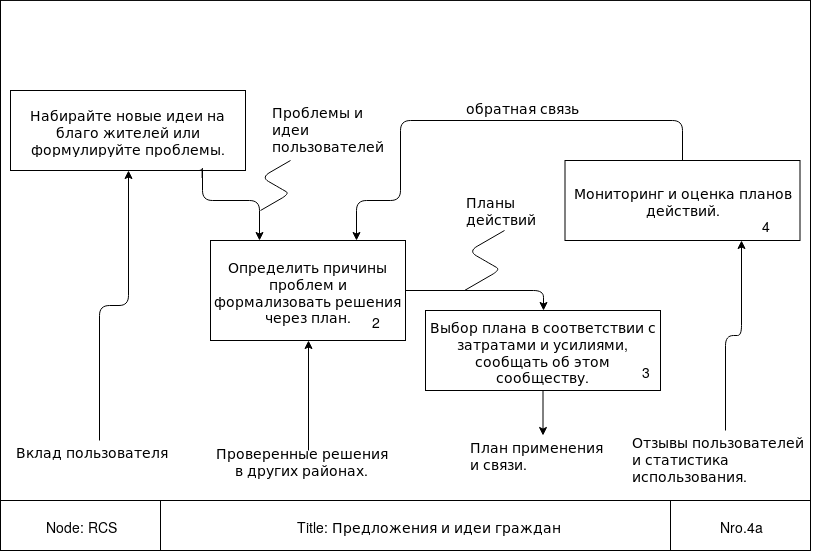
\includegraphics[scale=0.55]{diag4a.png}
  \caption{Структура системы Усовершенствования для соседства}
  \label{image:scheme12}
\end{figure}

\begin{table}[]
\centering
\begin{tabular}{|p{5cm}|p{5cm}|p{5cm}|}
\hline
\multicolumn{3}{|p{15cm}|}{Модульные улучшения для соседства (идеи пользователей)} \\ \hline

 Процесс  & Вход & Выход \\ \hline \hline
Набирайте новые идеи на благо жителей или формулируйте проблемы.& Вклад пользователя &
Проблемы и идеи пользователей\\ \hline
Определить причины проблем и формализовать решения через план. & Проблемы и идеи пользователей.& Планы действий. \\ \hline
Выбор плана в соответствии с затратами и усилиями, сообщать об этом сообществу. & Планы действий.& План применения и связи.\\ \hline
Мониторинг и оценка планов действий. & Отзывы пользователей и статистика использования. & Идеи на благо жителей района.\\ \hline
\end{tabular}
\centering
\caption{Процессы, связанные с улучшением окрестности.}
\centering
\label{tabla:sencilla2}
\end{table}







